\documentclass[10pt,a4paper,landscape]{article}
\usepackage[margin=15mm]{geometry}
\usepackage[T1]{fontenc}\usepackage{tgheros,textcomp}
\renewcommand{\familydefault}{\sfdefault}
\usepackage{xcolor,tikz,hyperref}
\definecolor{navy}{HTML}{171717}\definecolor{teal}{HTML}{242424}
\definecolor{gold}{HTML}{A0A0A0}\definecolor{pale}{HTML}{F2F2F2}
\hypersetup{colorlinks=true,urlcolor=teal,pdftitle={AquaShift business model canvas},pdfauthor={Loucas Louka; AquaShift team}}
\pagestyle{empty}\setlength{\parindent}{0pt}\color{navy}
\newcommand{\cell}[7]{\node[anchor=north west,draw=teal!25,fill=#6,rounded corners=0mm,inner sep=5mm,text width=#4cm,minimum height=#5cm,align=left] at (#1,#2) {\textbf{\color{teal}#3}\par\vspace{3mm}\small #7};}
\begin{document}
{\small\color{teal} AQUASHIFT \hfill PAFOS 2.0 / BUSINESS MODEL TO TEST}
\vspace{7mm}

{\fontsize{27}{31}\selectfont\bfseries Use the solar. Store the water.}\par
\vspace{3mm}
{\small Grid: desalination using otherwise curtailed solar. Sites: garden water budgets and overnight leak alerts.}

\vspace{6mm}
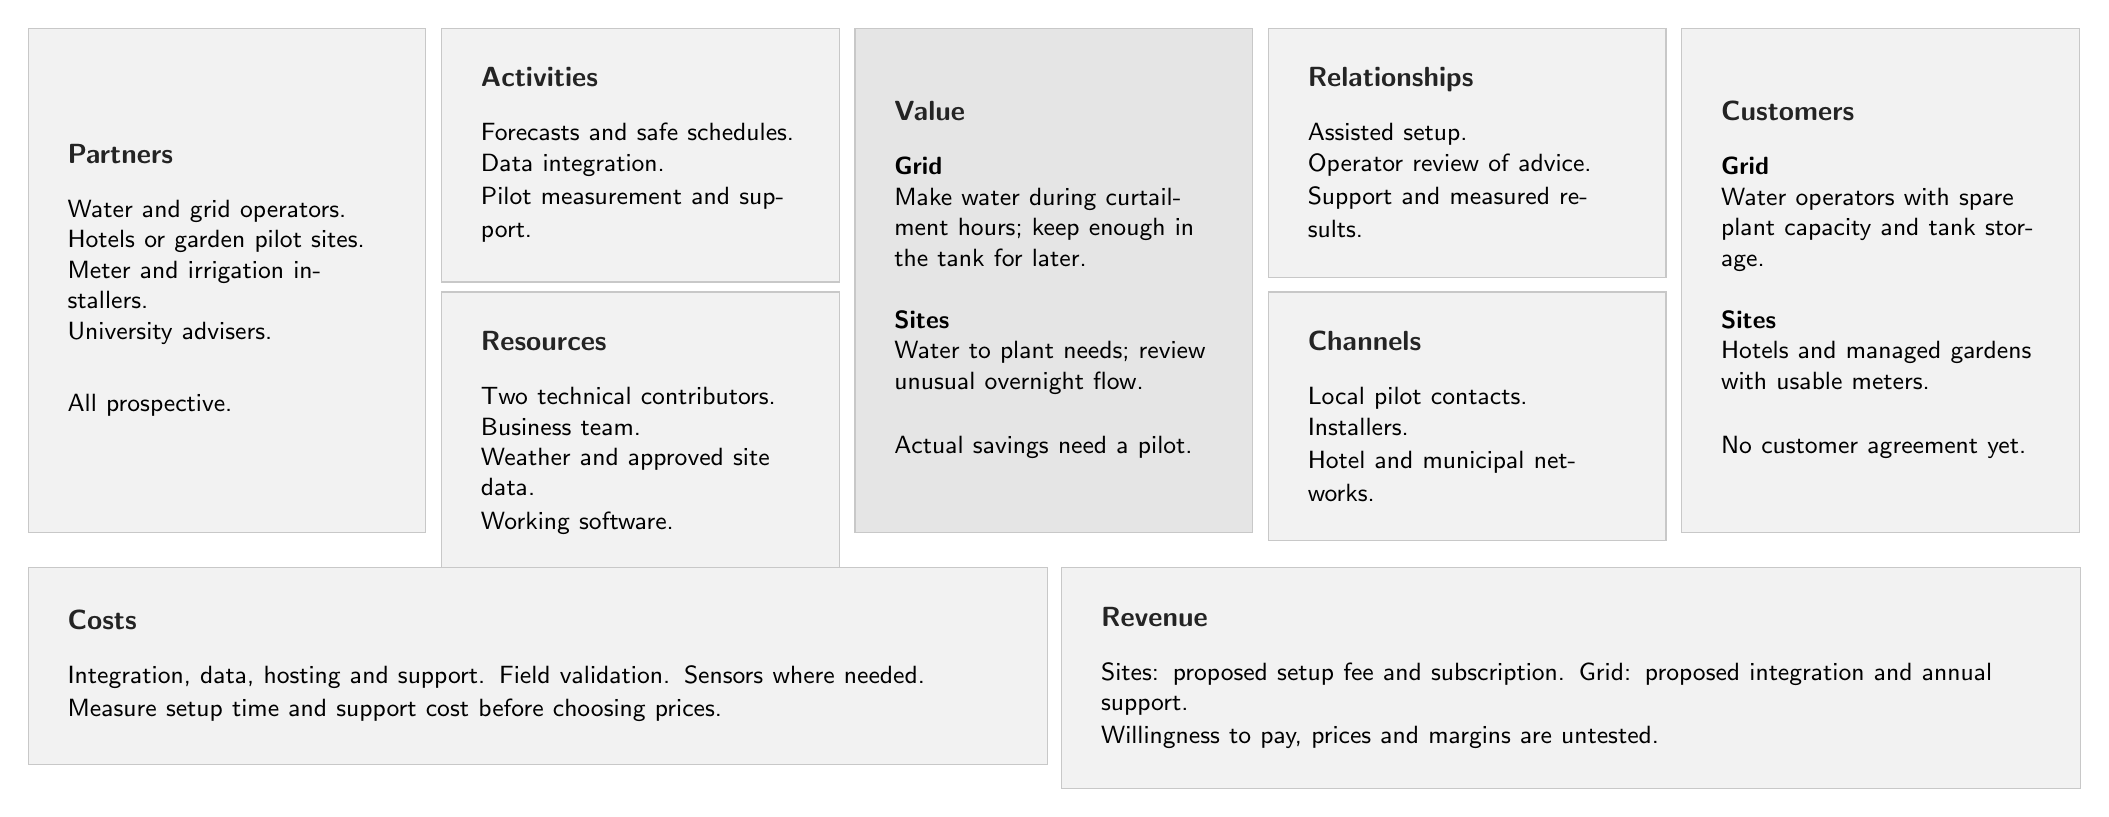
\begin{tikzpicture}[x=1cm,y=1cm]
\cell{0}{0}{Partners}{4.05}{6.4}{pale}{Water and grid operators.\par Hotels or garden pilot sites.\par Meter and irrigation installers.\par University advisers.\par\vspace{5mm}All prospective.}
\cell{5.25}{0}{Activities}{4.05}{3.1}{pale}{Forecasts and safe schedules.\par Data integration.\par Pilot measurement and support.}
\cell{5.25}{-3.35}{Resources}{4.05}{3.05}{pale}{Two technical contributors.\par Business team.\par Weather and approved site data.\par Working software.}
\cell{10.5}{0}{Value}{4.05}{6.4}{teal!12}{\textbf{Grid}\par Make water during curtailment hours; keep enough in the tank for later.\par\vspace{4mm}\textbf{Sites}\par Water to plant needs; review unusual overnight flow.\par\vspace{4mm}Actual savings need a pilot.}
\cell{15.75}{0}{Relationships}{4.05}{3.1}{pale}{Assisted setup.\par Operator review of advice.\par Support and measured results.}
\cell{15.75}{-3.35}{Channels}{4.05}{3.05}{pale}{Local pilot contacts.\par Installers.\par Hotel and municipal networks.}
\cell{21}{0}{Customers}{4.05}{6.4}{pale}{\textbf{Grid}\par Water operators with spare plant capacity and tank storage.\par\vspace{4mm}\textbf{Sites}\par Hotels and managed gardens with usable meters.\par\vspace{4mm}No customer agreement yet.}
\cell{0}{-6.85}{Costs}{11.94}{2.5}{pale}{Integration, data, hosting and support. Field validation. Sensors where needed.\par Measure setup time and support cost before choosing prices.}
\cell{13.125}{-6.85}{Revenue}{11.94}{2.5}{pale}{Sites: proposed setup fee and subscription. Grid: proposed integration and annual support.\par Willingness to pay, prices and margins are untested.}
\end{tikzpicture}

\vfill
{\footnotesize Starting point for team review. Original concept and philosophy: Loucas Louka; roadmap development: Stefanos. Business review: Andreas Nikolaides and Cleopas Cleopa.\par
Codex assisted these drafts. The current Grid result uses weather and tariff scenarios; actual curtailment absorption remains unmeasured. Sources: AquaShift roadmap, pitch and retained results.}
\end{document}
